% Options for packages loaded elsewhere
\PassOptionsToPackage{unicode}{hyperref}
\PassOptionsToPackage{hyphens}{url}
\PassOptionsToPackage{dvipsnames,svgnames,x11names}{xcolor}
%
\documentclass[
  letterpaper,
  DIV=11,
  numbers=noendperiod]{scrartcl}

\usepackage{amsmath,amssymb}
\usepackage{iftex}
\ifPDFTeX
  \usepackage[T1]{fontenc}
  \usepackage[utf8]{inputenc}
  \usepackage{textcomp} % provide euro and other symbols
\else % if luatex or xetex
  \usepackage{unicode-math}
  \defaultfontfeatures{Scale=MatchLowercase}
  \defaultfontfeatures[\rmfamily]{Ligatures=TeX,Scale=1}
\fi
\usepackage{lmodern}
\ifPDFTeX\else  
    % xetex/luatex font selection
\fi
% Use upquote if available, for straight quotes in verbatim environments
\IfFileExists{upquote.sty}{\usepackage{upquote}}{}
\IfFileExists{microtype.sty}{% use microtype if available
  \usepackage[]{microtype}
  \UseMicrotypeSet[protrusion]{basicmath} % disable protrusion for tt fonts
}{}
\makeatletter
\@ifundefined{KOMAClassName}{% if non-KOMA class
  \IfFileExists{parskip.sty}{%
    \usepackage{parskip}
  }{% else
    \setlength{\parindent}{0pt}
    \setlength{\parskip}{6pt plus 2pt minus 1pt}}
}{% if KOMA class
  \KOMAoptions{parskip=half}}
\makeatother
\usepackage{xcolor}
\usepackage{svg}
\setlength{\emergencystretch}{3em} % prevent overfull lines
\setcounter{secnumdepth}{-\maxdimen} % remove section numbering
% Make \paragraph and \subparagraph free-standing
\ifx\paragraph\undefined\else
  \let\oldparagraph\paragraph
  \renewcommand{\paragraph}[1]{\oldparagraph{#1}\mbox{}}
\fi
\ifx\subparagraph\undefined\else
  \let\oldsubparagraph\subparagraph
  \renewcommand{\subparagraph}[1]{\oldsubparagraph{#1}\mbox{}}
\fi


\providecommand{\tightlist}{%
  \setlength{\itemsep}{0pt}\setlength{\parskip}{0pt}}\usepackage{longtable,booktabs,array}
\usepackage{calc} % for calculating minipage widths
% Correct order of tables after \paragraph or \subparagraph
\usepackage{etoolbox}
\makeatletter
\patchcmd\longtable{\par}{\if@noskipsec\mbox{}\fi\par}{}{}
\makeatother
% Allow footnotes in longtable head/foot
\IfFileExists{footnotehyper.sty}{\usepackage{footnotehyper}}{\usepackage{footnote}}
\makesavenoteenv{longtable}
\usepackage{graphicx}
\makeatletter
\def\maxwidth{\ifdim\Gin@nat@width>\linewidth\linewidth\else\Gin@nat@width\fi}
\def\maxheight{\ifdim\Gin@nat@height>\textheight\textheight\else\Gin@nat@height\fi}
\makeatother
% Scale images if necessary, so that they will not overflow the page
% margins by default, and it is still possible to overwrite the defaults
% using explicit options in \includegraphics[width, height, ...]{}
\setkeys{Gin}{width=\maxwidth,height=\maxheight,keepaspectratio}
% Set default figure placement to htbp
\makeatletter
\def\fps@figure{htbp}
\makeatother

\KOMAoption{captions}{tableheading}
\makeatletter
\@ifpackageloaded{caption}{}{\usepackage{caption}}
\AtBeginDocument{%
\ifdefined\contentsname
  \renewcommand*\contentsname{Table of contents}
\else
  \newcommand\contentsname{Table of contents}
\fi
\ifdefined\listfigurename
  \renewcommand*\listfigurename{List of Figures}
\else
  \newcommand\listfigurename{List of Figures}
\fi
\ifdefined\listtablename
  \renewcommand*\listtablename{List of Tables}
\else
  \newcommand\listtablename{List of Tables}
\fi
\ifdefined\figurename
  \renewcommand*\figurename{Figure}
\else
  \newcommand\figurename{Figure}
\fi
\ifdefined\tablename
  \renewcommand*\tablename{Table}
\else
  \newcommand\tablename{Table}
\fi
}
\@ifpackageloaded{float}{}{\usepackage{float}}
\floatstyle{ruled}
\@ifundefined{c@chapter}{\newfloat{codelisting}{h}{lop}}{\newfloat{codelisting}{h}{lop}[chapter]}
\floatname{codelisting}{Listing}
\newcommand*\listoflistings{\listof{codelisting}{List of Listings}}
\makeatother
\makeatletter
\makeatother
\makeatletter
\@ifpackageloaded{caption}{}{\usepackage{caption}}
\@ifpackageloaded{subcaption}{}{\usepackage{subcaption}}
\makeatother
\ifLuaTeX
  \usepackage{selnolig}  % disable illegal ligatures
\fi
\usepackage{bookmark}

\IfFileExists{xurl.sty}{\usepackage{xurl}}{} % add URL line breaks if available
\urlstyle{same} % disable monospaced font for URLs
\hypersetup{
  pdftitle={From Smoke to Solution: Advancing Black Carbon as a Regulatory Pollutant},
  pdfauthor={Saloni Vijay},
  colorlinks=true,
  linkcolor={blue},
  filecolor={Maroon},
  citecolor={Blue},
  urlcolor={Blue},
  pdfcreator={LaTeX via pandoc}}

\title{From Smoke to Solution: Advancing Black Carbon as a Regulatory
Pollutant}
\author{Saloni Vijay}
\date{2024-07-16}

\begin{document}
\maketitle

\renewcommand*\contentsname{Table of contents}
{
\hypersetup{linkcolor=}
\setcounter{tocdepth}{3}
\tableofcontents
}
\href{https://creativecommons.org/licenses/by/4.0/}{\includesvg{index_files/mediabag/License-CC_BY_4.0-li.svg}}
\href{https://doi.org/10.5281/zenodo.12705811}{\includesvg{index_files/mediabag/zenodo.12705811.svg}}

\subsection{What is Black Carbon?}\label{what-is-black-carbon}

Black carbon is an air pollutant: a component of fine particulate matter
that is smaller than 2.5 mm in diameter (PM\textsubscript{2.5}), it is
formed through the incomplete combustion of
\href{https://www.ccacoalition.org/short-lived-climate-pollutants/black-carbon}{fossil
fuels, biomass, and waste}. Essentially, it is a very small particle
that forms part of a smoke plume that is either inhaled or dispersed
into the atmosphere.

\begin{figure}[H]

{\centering 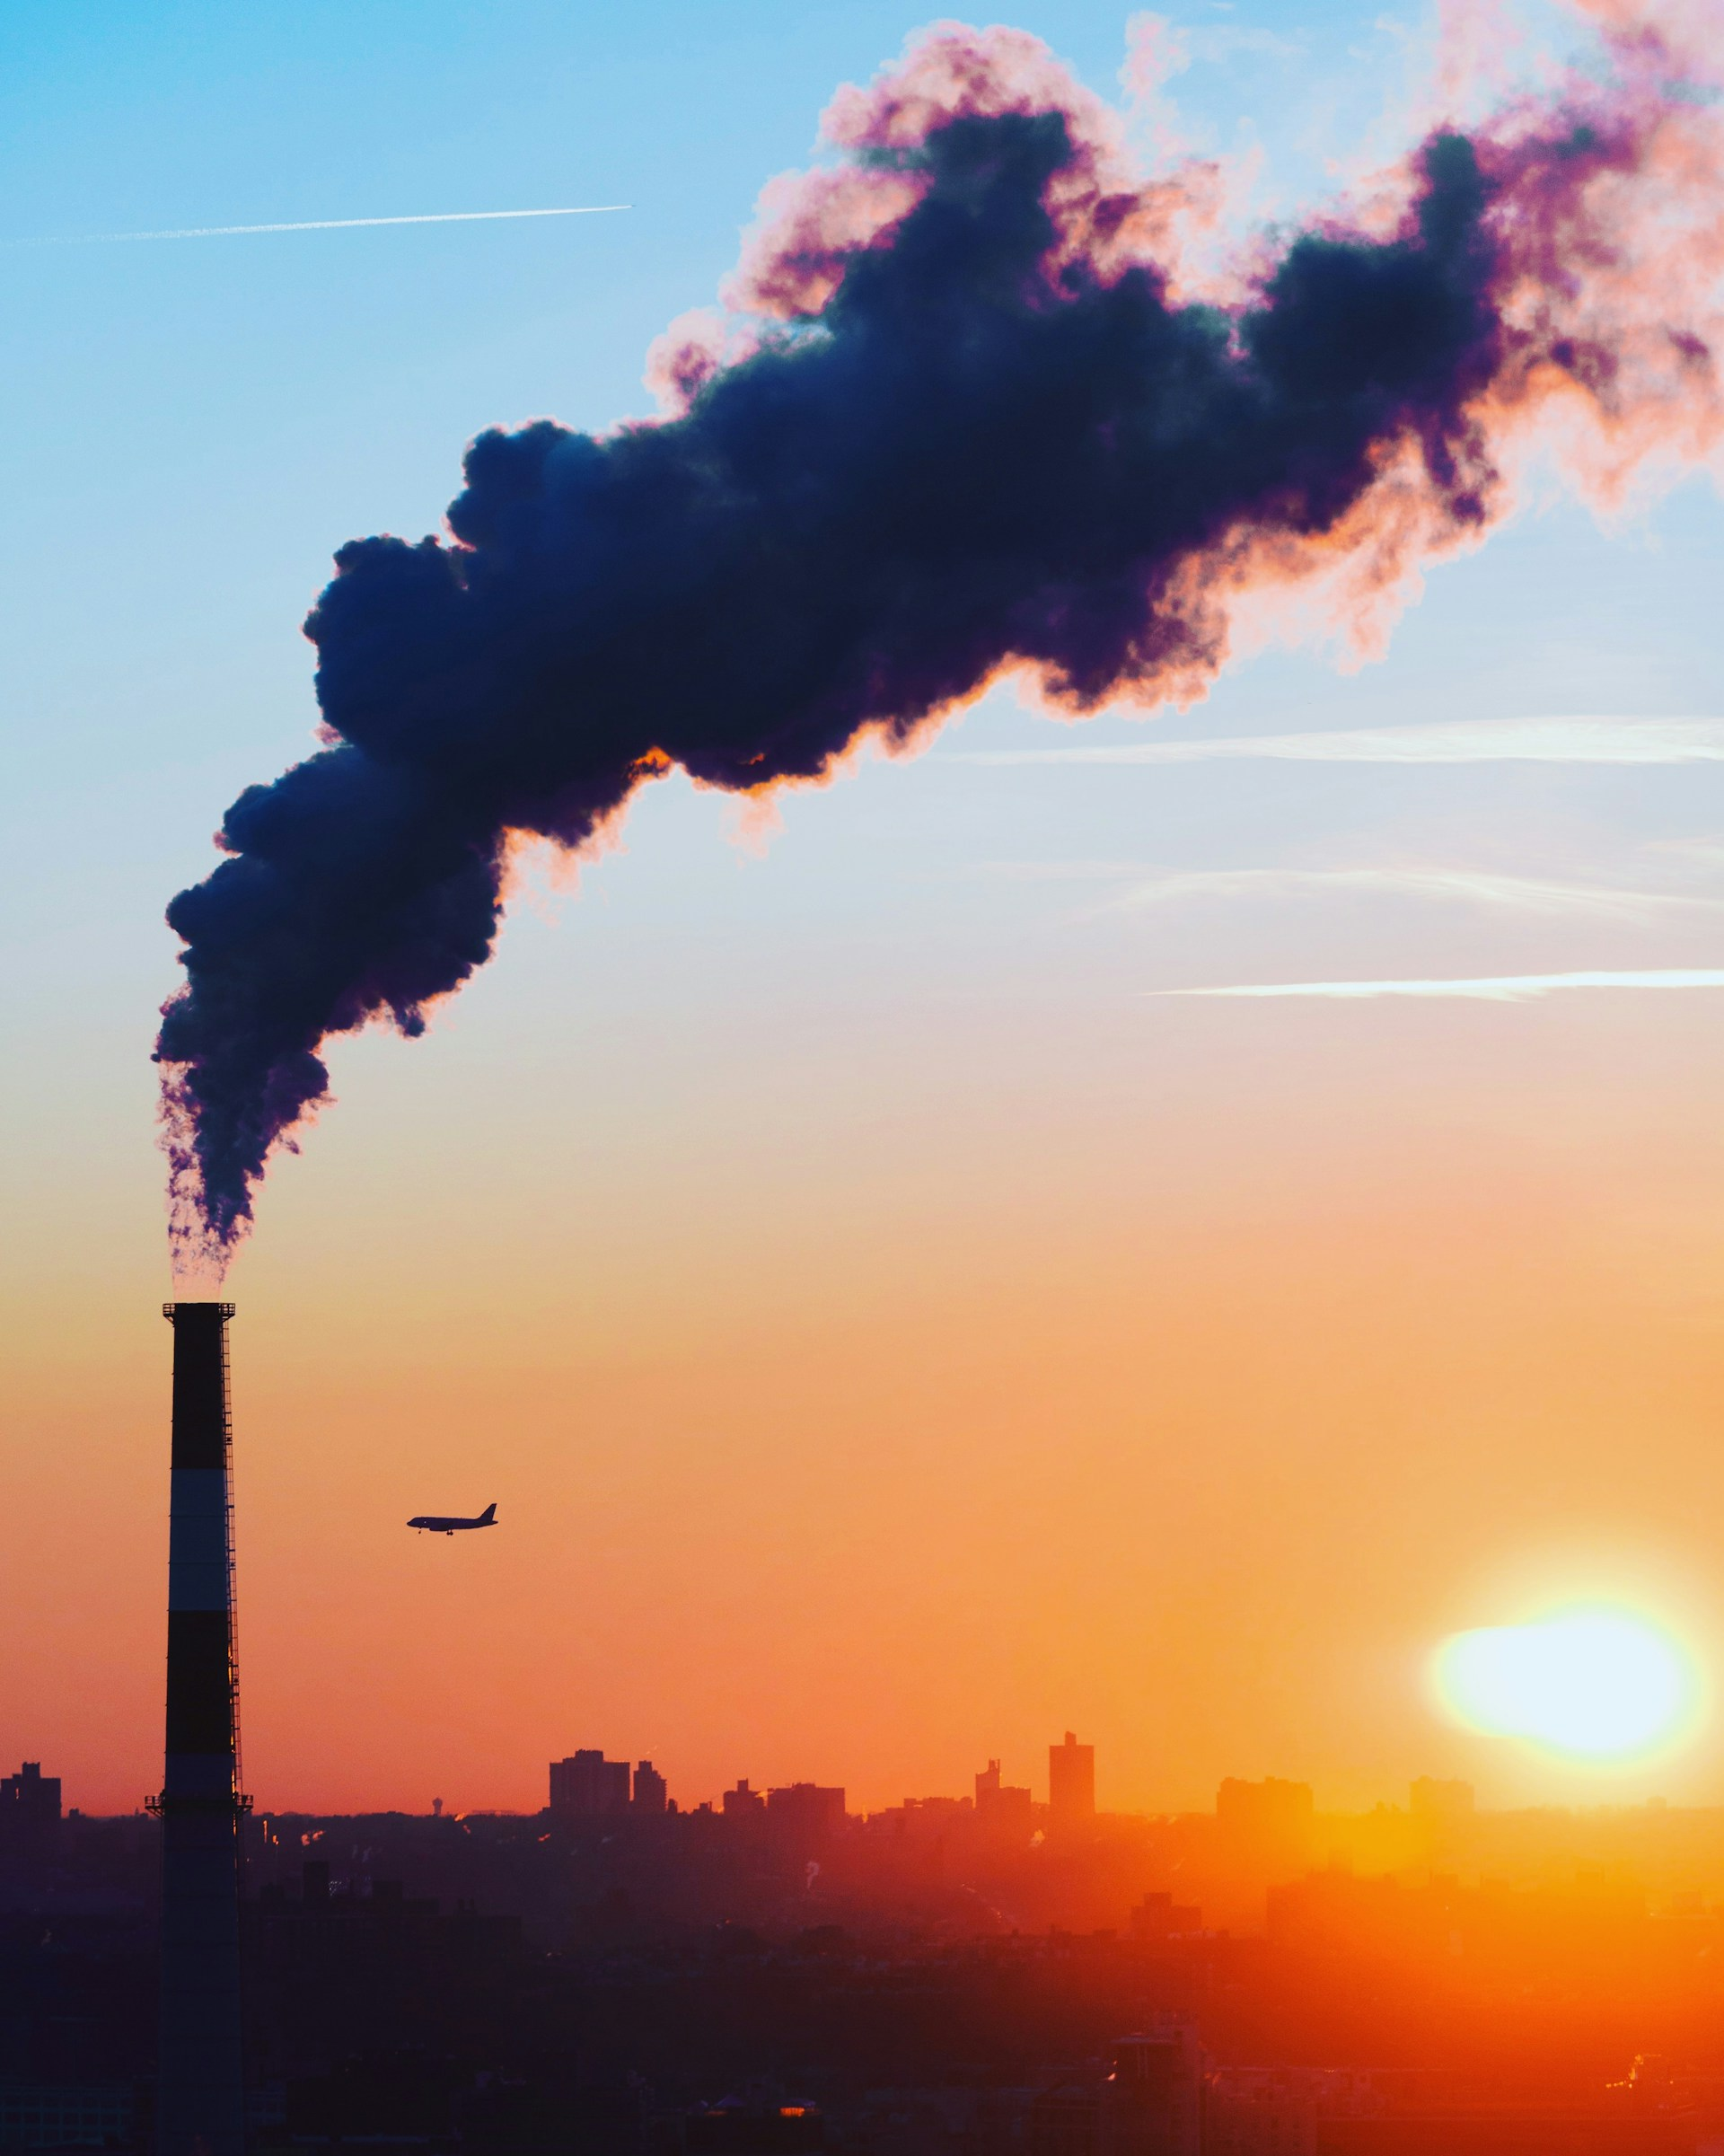
\includegraphics[width=6.4in,height=\textheight]{img/thijs-stoop-A_AQxGz9z5I-unsplash.jpg}

}

\caption{Black carbon, a sooty particulate matter in emission plumes.
Photo by
\href{https://unsplash.com/photos/white-smoke-A_AQxGz9z5I}{Thijs Stoop}
on \href{https://unsplash.com/}{Unsplash}.}

\end{figure}%

\subsection{The Case for Regulation}\label{the-case-for-regulation}

Due to its significant climate and health impacts, as well as its
traceability to specific sources, black carbon is increasingly discussed
as a potential regulatory pollutant.

\textbf{Climate Impacts:} Black carbon emissions are of concern due to
their extremely high global warming potential:
\href{https://en.wikipedia.org/wiki/Open_burning_of_waste}{up to 5000
times greater than CO\textsubscript{2}}. Black carbon absorbs sunlight
and heats the atmosphere, accelerating global warming. When deposited on
ice and snow, it reduces their reflectivity,
\href{https://www.ccacoalition.org/short-lived-climate-pollutants/black-carbon}{leading
to quicker melting}.

\textbf{Health Impacts:} These minute particles penetrate deep into the
lungs and enter the bloodstream, exacerbating respiratory and
cardiovascular diseases and increasing the risk of lung cancer. A
specific form of PM\textsubscript{2.5}, it is
\href{https://iris.who.int/bitstream/handle/10665/352615/9789289002653-eng.pdf?sequence=1}{more
toxic to human health} than other types of PM\textsubscript{2.5} such as
dust.

\textbf{Source Identification:} One reason why black carbon would be
easier to regulate than other pollutants is our ability to
\href{https://iris.who.int/bitstream/handle/10665/352615/9789289002653-eng.pdf?sequence=1}{pinpoint
the source.} Black carbon from fossil fuels and biomass can be
distinguished by their optical properties, allowing for targeted
reduction strategies. This capability enhances the effectiveness of
emission reduction efforts, enabling evidence-based decisions to address
the predominant sources.

\subsubsection{\texorpdfstring{\textbf{Gaps in Global Monitoring: The
case of
Africa}}{Gaps in Global Monitoring: The case of Africa}}\label{gaps-in-global-monitoring-the-case-of-africa}

Despite the significant climate and health impacts of black carbon,
global monitoring efforts remain inadequate. While ambient black carbon
monitoring is
\href{https://www.clarity.io/blog/air-quality-measurements-series-black-carbon}{increasing
in European countries}, the United States,
\href{https://mausam.imd.gov.in/imd_latest/contents/environmental-monitoring-services.php}{India}
and \href{https://www.mdpi.com/2073-4433/11/7/684}{China}, but Africa
lags behind. Only a few countries, such as
\href{https://www.sciencedirect.com/science/article/pii/S0048969723011981}{Ghana},
\href{https://www.nature.com/articles/s43247-022-00400-1}{Kenya}, and
\href{https://www.sciencedirect.com/science/article/abs/pii/S2212095522002309\#:~:text=Only\%20two\%20studies\%20of\%20BC,et\%20al.\%2C\%202020}{Rwanda}.),
have some ambient black carbon data, with the high cost of monitors
being a major barrier to more extensive data collection.

Even PM\textsubscript{2.5}, which was declared a regulatory pollutant in
1997 in the U.S., is still inadequately monitored in many African
countries. Western Africa has approximately one
reference-grade\footnote{A reference-grade air quality monitor is a
  high-precision, certified instrument used for accurate and reliable
  measurements of air pollutants, meeting stringent regulatory
  standards.} PM\textsubscript{2.5} monitor per 10 million people, and
the situation is even worse in Eastern Africa, with only
\href{https://scielo.org.za/scielo.php?script=sci_arttext&pid=S2410-972X2021000100009\#:~:text=In\%20Western\%20Africa\%2C\%20there\%20is,et\%20al.\%2C\%202020}{one
reference-grade monitor per 100 million people}.). Introducing black
carbon as a regulatory pollutant would require substantial investment
and infrastructure development to achieve effective monitoring across
the continent. Figure~\ref{fig-openaq} illustrates the global
distribution of PM2.5 monitoring stations, as documeted by
OpenAQ\footnote{OpenAQ is a nonprofit organization providing universal
  access to air quality data to empower a global community of
  changemakers to solve air inequality---the unequal access to clean
  air.}.

\begin{figure}

\centering{

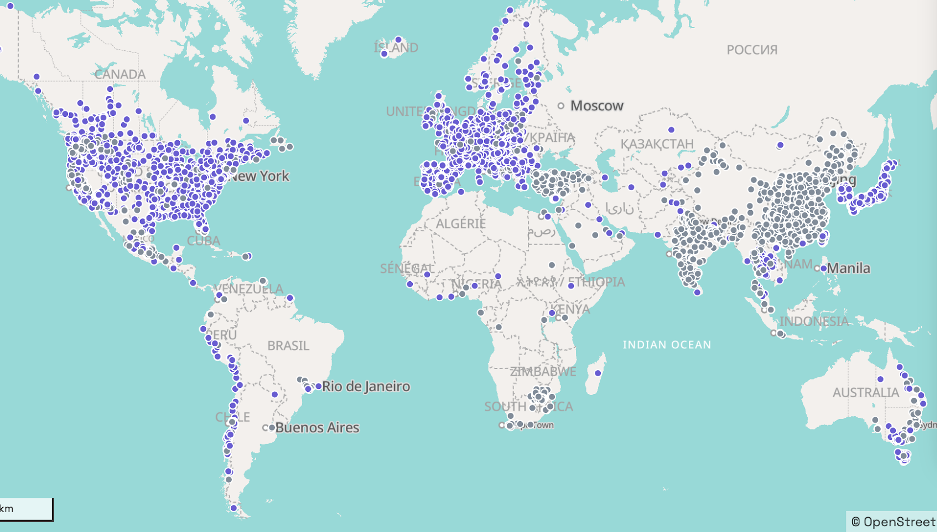
\includegraphics[width=3.13in,height=\textheight]{img/screenshot-openaq.png}

}

\caption{\label{fig-openaq}A screenshot from OpenAQ illustrating the
global distribution of PM2.5 monitoring stations.}

\end{figure}%

\subsection{Overcoming Cost Barriers: Innovating Affordable
Solutions}\label{overcoming-cost-barriers-innovating-affordable-solutions}

Low-cost PM\textsubscript{2.5} monitors have expanded access to air
quality data. We need similar advancements for black carbon monitoring.
Developing hybrid networks that integrate low-cost monitors with
reference-grade stations could enhance coverage and accuracy. Currently,
what is considered cost-effective
\href{https://metone.com/introducing-the-groundbreaking-c-12-portable-carbon-monitor-making-carbon-measurements-accessible-worldwide/}{often
exceeds 3000 USD}. During my PhD research in
\href{https://en.wikipedia.org/wiki/Malawi}{Malawi}, I utilized the
\href{https://aethlabs.com/microaeth/ma200/overview}{microAeth\textsuperscript{®}
MA200} monitor for personal exposure measurements, which, while less
costly than other monitors, was still expensive for the low-income
context. Each filter tape, costing approximately 100 USD, lasted only
three days due to the high-concentration environment, underscoring the
ongoing financial challenges in resource-limited settings.

Research efforts are crucial to developing affordable monitoring
technology, particularly in regions like
\href{https://www.clarity.io/blog/air-quality-measurements-series-black-carbon\#:~:text=More\%20than\%2075\%25\%20of\%20global,lack\%20comprehensive\%20air\%20quality\%20regulations.}{Asia
and Africa that contribute 63\% of global black carbon emissions}.
Current monitors, primarily designed for cleaner environments, are
inadequate for high-emission areas; even after the initial investment,
recurring costs such as filter tapes continue to pose challenges.

\begin{figure}[H]

{\centering 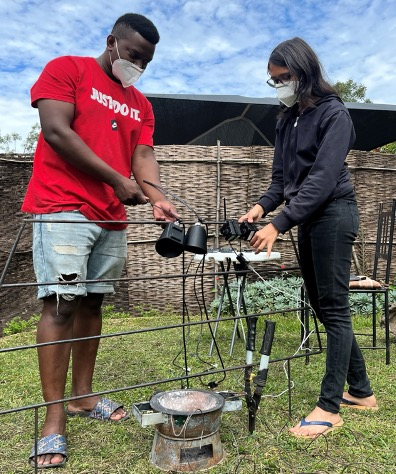
\includegraphics[width=1.32in,height=\textheight]{img/measuring-air-quality.jpg}

}

\caption{Saloni Vijay, the author of this blog (right), and Hope Kelvin
Chilunga (left), a collaborator of the GHE group, setting up an
experiment to monitor black carbon emissions from cooking with solid
biofuels in Blantyre, Malawi. Photo by Saloni Vijay,
\href{https://creativecommons.org/licenses/by/4.0/deed.en}{CC-BY}
license.}

\end{figure}%

\subsection{Navigating Ambient Concentrations: The Need for
Standards}\label{navigating-ambient-concentrations-the-need-for-standards}

In \href{https://visitmalawi.mw/index.php/blantyre-city/}{Blantyre,
Malawi}, the average black carbon concentration was 3.85
μg/m\textsuperscript{3} in July-August 2023. Without established
regulatory standards, interpreting such figures remains challenging.
While black carbon monitoring has seen recent advancements, questions
persist: Are these concentrations safe?

While no national or international air quality standards for black
carbon exist yet, both the
\href{https://fpi.ec.europa.eu/news/eu-action-sheds-light-black-carbon-emissions-2019-08-27_en}{European
Union} and the
\href{https://iris.who.int/bitstream/handle/10665/352615/9789289002653-eng.pdf?sequence=1}{World
Health Organization} have recognized its significant threats to health
and climate. This acknowledgment suggests
\href{https://en.ilmatieteenlaitos.fi/tiedote/5ePGJSjeZo1t5qvIjQO992}{impending
regulations on black carbon emissions and air quality standards.}

\begin{figure}

\begin{minipage}{0.35\linewidth}

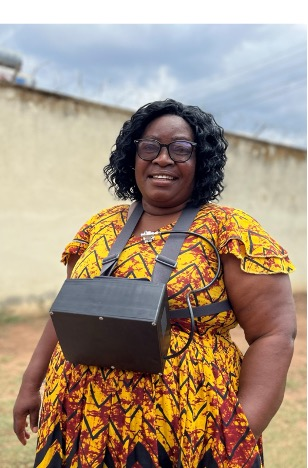
\includegraphics{img/personal-monitor.jpg}

\subcaption{\label{}A volunteer wears a personal monitor for Saloni's
PhD project on black carbon exposure. Photo by Saloni Vijay,
\href{https://creativecommons.org/licenses/by/4.0/deed.en}{CC-BY}
license.}
\end{minipage}%
%
\begin{minipage}{0.04\linewidth}
~\end{minipage}%
%
\begin{minipage}{0.61\linewidth}

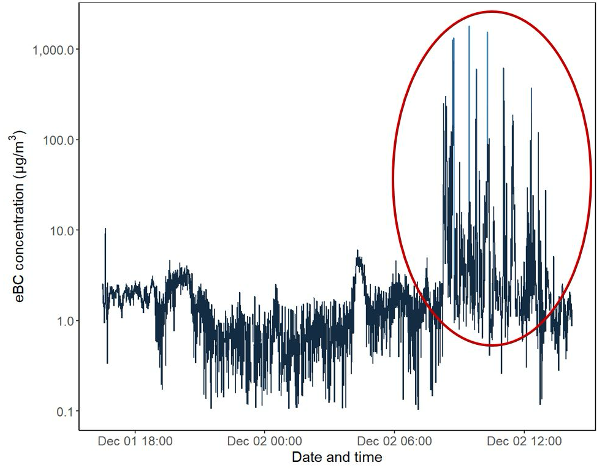
\includegraphics{img/plot-measurements.png}

\subcaption{\label{}Personal exposure to black carbon in Blantyre,
Malawi, during the burning of garden waste. The red oval indicates the
burning period. Because there are no regulatory limits on ambient air
concentrations, the risks are unclear.}
\end{minipage}%

\end{figure}%

\subsection{Steps Forward}\label{steps-forward}

Effective black carbon regulation requires a multifaceted approach that
includes technological, regulatory, and educational initiatives.

\textbf{Develop Affordable Monitors:}~To make black carbon regulation
feasible, affordable and reliable monitoring technology must be
developed. Investment in research and the development of low-cost
monitors is essential to facilitate widespread adoption.

\textbf{Establish Clear Guidelines} \textbf{for Monitoring and
Reporting:} These guidelines should be internationally harmonized to
ensure consistency and comparability of data. Additionally, proper
limits for ambient concentrations need to be established to provide
clear standards for assessing black carbon levels and their impacts.

\textbf{Raise Awareness and Build Capacity}:~This includes training and
resources for local authorities to implement and maintain monitoring
networks.

\textbf{Policy Integration:}~ Leveraging existing infrastructure and
expertise from PM\textsubscript{2.5} monitoring could accelerate the
implementation of black carbon regulations.

By addressing these key areas, we can enhance our ability to monitor,
regulate, and reduce black carbon concentrations, ultimately improving
air quality and public health.

\subsection{About the author}\label{about-the-author}

\href{https://www.linkedin.com/in/saloni-vijay-9b9a51a7/}{Saloni Vijay}
is a PhD student in the Global Health Engineering group, ETH Zurich. She
is currently focused on evaluating the environmental risks and health
impacts of open trash burning, with a specific emphasis on black carbon
concentrations in Blantyre, Malawi.

If you are interested in learning more about Saloni's work on Black
Carbon in Blantyre, feel free to write her an email at
\href{mailto:svijay@ethz.ch}{\nolinkurl{svijay@ethz.ch}} or on
\href{https://www.linkedin.com/in/saloni-vijay-9b9a51a7/}{LinkedIn}.

Saloni is giving a talk at the \href{https://www.eac2024.fi/}{European
Aerosol Conference, 2024 in August in Tampere, Finland}, and attending
the \href{https://icacgp-igac2024.com/}{International Global Atmospheric
Chemistry (IGAC) short course and conference, 2024 in September in
Malaysia}. If you are present at any of these events, please reach out
and connect. She would love to hear about your work and share hers.



\end{document}
